% !TeX spellcheck = ru_RU
\documentclass[specialist,
substylefile = spbu_report.rtx,
subf,href,colorlinks=true, 12pt]{disser}

\usepackage{amsmath,amssymb,amsthm,amscd,amsfonts,mathabx}
\usepackage[utf8]{inputenc}
\usepackage[a4paper,
left=2cm, right=1.5cm, top=2cm, bottom=2cm]{geometry}
\usepackage{graphicx}
\usepackage[russian]{babel}
\usepackage{xcolor}
\usepackage{float}

\setcounter{tocdepth}{3}
\setcounter{secnumdepth}{3}


\newtheorem{defenition}{Определение}

\begin{document}
	\institution{%
		Санкт-Петербургский государственный университет\\
		Прикладная математика и информатика
	}
	
	\title{Отчет по Научно-исследовательской работе}	
	\topic{Задачи оценивания значимости выравнивания при помощи скрытых марковских моделей}	
	\author{Власенко Даниил Владимирович}
	\group{группа 19.Б04-мм}
	\sa{Коробейников Антон Иванович\\
		Кафедра Статистического Моделирования}
	\sastatus {д.\,ф.-м.\,н., профессор}	
	\city{Санкт-Петербург}
	\date{\number\year}	
	\maketitle
	\tableofcontents
	
	
	\intro
		Пусть дан алфавит символов $\Sigma$. 
		\begin{defenition}Последовательностью длины $L$ над алфавитом $\Sigma$ будем называть такой $X$, что $X \in \Sigma^{L}$. Последовательностью $X$ над алфавитом $\Sigma$ будем называть такой $X$, что $X \in \bigcup_{L=0}^{L=\infty}\Sigma^{L}$.
		\end{defenition}
		
		Сходство последовательностей может отражать функциональные, структурные или эволюционные взаимосвязи объектов, которые описывают эти последовательности. Таким образом умение находить взаимосвязи в строках может быть приложимо в задаче определения степени родства биологических организмов путем сравнения их ДНК или РНК, нуклеотидных последовательностей, задаче анализа свойств белков, аминокислотных последовательностей, задаче распознавания речи человека или письменного языка и многих других приложениях. 
		
		\begin{defenition}
			Выравниванием $N$ последовательностей называется отображение \\$Q: \bigtimes_{i=1}^{N}(\bigcup_{L_i=0}^{\infty} \Sigma^{L_i}) \rightarrow \bigtimes_{i=1}^{N}(\Sigma^{L})$, где $L = \max(\{L_i\}_{i=1}^{N})$ такое что:
			\begin{enumerate}
				\item Возможны вставки символа --- в последовательностях.
				\item Вставка --- на одинаковых позициях во всех последовательностях запрещена.
				\item Порядок изначальных символов внутри последовательностей сохраняется.
			\end{enumerate}
		\end{defenition}		
		
		Элементы из области значения $Q$ также называются выравниваниями. Примем множество $\bigtimes_{i=1}^{N}(\bigcup_{L_i=0}^{L_i=\infty} \Sigma^{L_i})$ за пространство элементарных исходов $\Omega$. Область значений выравнивания $Q$ обозначим как $\overline \Omega$.
		
		\begin{figure}[H]
			\centering
			\begin{tabular}{cccccccc}
				A&C&E&A&A&F&A&E\\
				C&E&A&F&D&C&E&
			\end{tabular}
		\end{figure}
		\begin{figure}[H]
			\centering
			\begin{tabular}{ccccccccc}
				A&C&E&A&A&F&A&—&E\\
				—&C&E&A&—&F&D&C&E
			\end{tabular}
			\caption{Последовательности до и после выравнивания.} \label{fg:1}
		\end{figure}
		
		\begin{defenition}				
			Оценкой выравнивания называется случайная величина $s:\overline \Omega \rightarrow \mathbb{R}$.
		\end{defenition}	
		
		Способом вычисления оценки выравнивания $s$ может быть, например, увеличение оценки на 1 при совпадении символов, стоящих на одинаковых позициях в последовательностях, и уменьшение на $\frac{1}{2}$ при несовпадении. Тогда оценка $s$ приведенного на рисунке~\ref{fg:1} выравнивания будет равна 3.
						
		Определить оценку выравнивания можно разными способами, но смысл будет иметь такое определение, чтобы оценка была мерой того, насколько сильно строки выравнивания похожи друга на друга.
		
		Пусть даны последовательности $\{X_i\}_{i=1}^{N}$ и задана оценка выравнивания $s$. Тогда задача оценки сходства последовательностей $\{X_i\}_{i=1}^{N}$ сводится к решению оптимизационной задачи:		
		\begin{equation*}
			\max_{\overline{\omega} \in \overline{\Omega} : Q(\{X_i\}_{i=1}^{N}) = \overline{\omega}}s(\overline{\omega}). \label{eq:1}
		\end{equation*}	
	
		Предположим, что даны последовательность $X$ и выравнивание $\omega \in \overline{\Omega}$ из $N$ строк. 
				
		\begin{defenition}
			Выравниванием последовательности $X$ к выравниванию $w$ называется отображение $\boldsymbol{Q}: (X, \overline{\Omega}) \rightarrow \bigtimes_{i=1}^{N+1}(\Sigma^{L})$, где $L = \max(\{L_i\}_{i=1}^{N+1})$ такое что:
			\begin{enumerate}
				\item Возможны вставки символа --- в последовательностях.
				\item Вставка --- на одинаковых позициях во всех последовательностях запрещена.
				\item Порядок изначальных символов внутри последовательностей сохраняется.
			\end{enumerate}
		\end{defenition}
		
		Примем множество $(\Omega, \overline \Omega)$ за пространство элементарных исходов $\boldsymbol{\Omega}$. Область значений выравнивания $\boldsymbol Q$ обозначим как $\overline{\boldsymbol{\Omega}}$.
		
		\begin{defenition}				
			Оценкой выравнивания последовательности $X$ к выравниванию $w$ называется случайная величина $\boldsymbol s:\overline{\boldsymbol{\Omega}} \rightarrow \mathbb{R}$.
		\end{defenition}
	
		Пусть даны последовательность $X$, выравнивание $\overline{\omega} \in \overline{\Omega}$ и задана оценка выравнивания $\boldsymbol{s}$. Тогда задача оценки сходства последовательности $X$ и последовательностей, описываемых выравниванием $\overline{\omega}$, сводится к решению оптимизационной задачи:		
		\begin{equation*}
			\max_{\overline{\boldsymbol{\omega}} \in \overline{\boldsymbol{\Omega}} : \boldsymbol{Q}(X, \overline{\omega}) = \overline{\boldsymbol{\omega}}}s(\overline{\boldsymbol{\omega}}). \label{eq:2}
		\end{equation*}		
		Встает вопрос того, как интерпретировать решение этой задачи. 
		
		Пусть дана последовательность $X$, выравнивание $\overline{\omega} \in \overline{\Omega}$, задана оценка оценка выравнивания $\boldsymbol{s}$ и известно, что $\overline{\omega}$ построено на последовательностях, описывающих взаимосвязанные объекты.
		\begin{defenition}
			Шумом будем называть случайную последовательность над алфавитом $\Sigma$. Сигналом будем называть последовательность над алфавитом $\Sigma$, которая описывает объект, взаимосвязанный с объектами последовательностей, описываемых $\overline{\omega}$.
		\end{defenition}
		
		Достаточно ли низкая оценка $\boldsymbol{s}(X, \overline{\omega})$, чтобы считать последовательность $X$ шумом, или сигнал мог получить такую оценку?
		
	\chapter{Метод}
		Для ответа на поставленный вопрос сначала опишем нужные нам модели, затем алгоритмы, которые используются для манипуляции ими.
		\section{Модели}
			Метод предполагает, что даны профильная СММ, с помощью которой будут оцениваться последовательности, и фоновая модель $B$, которая будет описывать шум.
			\subsection{Скрытая марковская модель}
				\begin{defenition}
					Пусть $Z_{n}$ и $Y_{n}$ дискретные стохастические процессы, $n \geq 1$. Пара $(Z_{n}, Y_{n})$ называется скрытой марковской моделью, если
					\begin{itemize}
						\item $Z_{n}$~--- марковский процесс, поведение которого напрямую не наблюдается ("скрытый");
						\item $P(Y_{n} = y_{n}|Z_{1} = z_{1},\dots, Z_{n} = z_{n}) = P(Y_{n}|Z_{n}=z_{n})$ для любого $n \geq 1$, где $z_{1},\dots,z_{n}$~--- значения, принимаемые процессом  $Z_{n}$ (\textbf{состояния модели}), $ y_{n}$~--- значение, принимаемое процессом $Y_{n}$ (\textbf{наблюдаемый символ модели}).
					\end{itemize}
				\end{defenition}	
				
				\begin{defenition}
					Путем $\pi$ называется последовательность состояний $\{z_i\}_{i=1}^{n}$ и наблюдаемых символов $\{y_i\}_{i=1}^{n}$ СММ.
					Последовательность $X$, которая была получена в результате прохода СММ пути $\pi$, называется последовательностью наблюдаемых символов.
				\end{defenition}
				
				\begin{figure}[h]
					\centering
					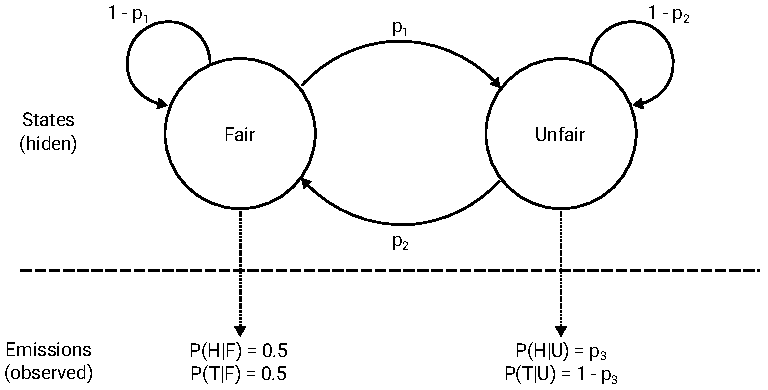
\includegraphics[width=12cm]{figure1}
					\caption{Простая скрытая марковская модель.} 
					\label{fg:2}
				\end{figure}
			
				Примером простой СММ может быть модель, изображенная на рисунке~\ref{fg:2} и описывающая подбрасывание двух монет. Пусть между наблюдателем и человеком с монетами стоит ширма, которая позволяет наблюдателю видеть только пол, куда падают монеты. Пусть есть две монеты: одна "--- честная монета, вторая "--- нечестная монета с перевесом в одну из сторон. Пусть человек с монетами с некоторой вероятностью либо подбрасывает монету, которую он бросил в прошлый раз, либо меняет монеты и бросает новую. При этом наблюдатель не знает, какая монета используется в конкретный момент времени, так как он не видит рук бросающего монеты и не может отличить одну монету от другой по их внешнему виду, он видит только последовательность результатов бросков.
				
			\subsection{Профильная скрытая марковская модель}
				Профильная СММ "--- это СММ со специальной линейной архитектурой состояний, которая позволяет выравнивать последовательность к множеству последовательностей~\cite{Compeau2015a}.
				
				\begin{figure}[h]
					\centering
					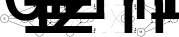
\includegraphics[width=15cm]{figure2}
					\caption{Профильная скрытая марковская модель.}  
					\label{fg:3}
				\end{figure}
				
				Пусть даны последовательность $X$ и выравнивание $\overline{\omega} \in \overline{\Omega}$.	Профильная СММ состоит из трех типов состояний, распределения которых строятся на основе $\overline{\omega}$:
				\begin{itemize}
					\item S-состояние --- начальное состояние,
					\item М-состояния --- устанавливают соответствие символов в $X$ и $\overline{\omega}$,
					\item I-состояния и D-состояния --- устанавливает соответствие пропуска и символа в $X$ и $\overline{\omega}$,
					\item E-состояние --- конечное состояние.
				\end{itemize}
			
				Алгоритмы профильных СММ позволяют по-разному оценивать выравнивание $X$ к  $\overline{\omega}$~\cite{Newberg2009, Compeau2015a}. 
				
				\begin{defenition}
					Вероятность пути $s(\pi)$ "--- произведение всех переходных вероятностей от состояний к состоянию и вероятностей наблюдаемых символов, которые излучаются в каждом состоянии, кроме начального и конечного, на протяжении всего пути $\pi$. 
				\end{defenition}
				
				Вероятность Витерби $s_{max}(X)$ последовательности $X$ "--- это максимальная вероятность последовательности $X$ среди всех путей $\pi$, которые могли бы ее испустить:
				\begin{equation*}
					s_{max}(X) = \underset{\pi \in \pi_{X}}{max}(s(\pi)),
					\label{eq:3}
				\end{equation*}
				Несмотря на большое количество возможных путей, которые могли бы испустить последовательность $X$, алгоритм Витерби позволяет эффективно решать эту задачу.
				
				Форвард вероятность $s_{fw}(X)$ последовательности $X$ "--- это общая вероятность того, что в результате работы СММ будет получена последовательность $X$:
				\begin{equation*}
					s_{fw}(X) = \sum_{\pi \in \pi_{X}}s(\pi).
					\label{eq:4}
				\end{equation*}		
				Форвард алгоритм работает за то же время, что и алгоритм Витерби.
				
				Третий способ оценивать последовательности, позволяющий уменьшить дисперсию дальнейших вычислений оценки ложноположительной вероятности оценки, заключается в том, что каждая вероятность перехода из одного состояния в другое и вероятность излучения символа состоянием будут возводится в степень $\frac{1}{T}$, где $T \in (0; +\infty)$. При этом логика вычислений остается та же, то есть $s(\pi)^{\frac{1}{T}}$ и $s(X)^{\frac{1}{T}}$ будут вычисляться как вероятность произведения независимых событий и как сумма непересекающихся событий соответственно, хотя они уже могут не являться вероятностями (Например, сумма всех $s(\pi)^\frac{1}{T}$ не обязательно равна единице):
				\begin{equation*}
					Z(X, T)	= \sum_{\pi \in \pi_{X}}s(\pi)^{\frac{1}{T}}.
					\label{eq:5}
				\end{equation*}		
				Функция $Z(X, T)$ называется статистической суммой и вычисляется через модификацию Форвард алгоритма. Параметр $T$ подбирается экспериментально под конкретную интересующую оценку выравнивания.
			\subsection{Фоновая модель}
				\begin{defenition}
					Моделью последовательностей называется генератор, моделирующий последовательности в соответствии с некоторым распределением. 
				\end{defenition}
				
				$P(X|M)$, где $M$ --- некоторая модель, означает условную вероятность $X$, при условии ее моделирования моделью $M$.
				
				\begin{defenition}
					Фоновой моделью $B$ для последовательностей длины $L$ называется генератор последовательностей длины $L$ такой, что все $L$ символьных позиций независимы и одинаково распределены:
					\begin{equation}
						\mathsf{P}(X|B) = \prod_{i=1}^{L}\mathsf{P}(x_{i}|B), \label{eq:6}
					\end{equation}
					где $x_i$ отражает возможный наблюдаемый символ.
				\end{defenition}
				
				Фоновая модель описывает шум.
				
			\subsection{Постановка математической задачи.}
				Последовательность $X$ длины $L$ сравнивается с остальными последовательностями той же длины.
				\begin{defenition}
					Ложноположительная вероятность оценки $s_{0}$ для строк длины $L$:	
					\begin{equation}
						fpr(s_{0}) =  \sum_{X \in X_{L}} \mathsf{P}(X|B) \Theta(s(X) \geq s_{0}), 
						\label{eq:7}
					\end{equation}
					где $\mathsf{P}(X|B)$ "--- условная вероятность последовательности $X$, описываемая фоновой моделью, $s(X)$ "--- оценка последовательности $X$, считаемая профильной СММ, и
					\[
					\Theta(s(X) \geq s_{0}) = 
					\begin{cases}
						1, & s(X) \geq s_{0}\\
						0, & s(X) < s_{0}
					\end{cases}.
					\]
				\end{defenition}	
				То есть $fpr(s_{0})$ "--- это вероятность того, что шум достигнет или превзойдет оценку $s_{0}$. В определении $fpr(s_{0})$ оценка $X$ отмечена как $s(X)$, потому что способ оценки последовательности может выбираться относительно интересующего приложения, подходит $s(X) = s_{max}(X)$ и $s(X) = s_{fw}(X)$.
			
		\section{Алгоритм}
			\subsection{Выборка по значимости}
				Так как вычисление $fpr(s_{0})$ по формуле~\eqref{eq:7} обычно неосуществимо, значение $fpr(s_{0})$ может быть оценено через выборку по значимости, то есть через моделирование строк в соответствии с фоновой моделью $B$ и оценивание значения $fpr(s_{0})$ долей тех из них, что достигают оценки $s_{0}$.
				
				Построим распределение, относительно которого будем моделировать строки. Пусть $\mathsf{P}(X|T)$ "--- это условная вероятность строки $X$ относительно некоторой модели строк длины $L$ параметризованной значением $T$. Тогда можно переписать $fpr(s_{0})$:
				\begin{equation*}
					fpr(s_{0}) = \sum_{X \in X_{L}} \mathsf{P}(X|T) f(X,s_{0}),
					\label{eq:8}
				\end{equation*}
				где
				\begin{equation}
					f(X,s_{0}) = \frac{\mathsf{P}(X|B) \Theta(s(X) \geq s_{0})}{\mathsf{P}(X|T)}.
					\label{eq:9}
				\end{equation}
				Мы можем оценить значение $fpr(s_{0})$ через моделирование последовательностей в соответствии с этой альтернативной моделью и подсчет среднего значения $f(X,s_{0})$. Этот подход и называется выборкой по значимости, он полезен, потому что если правильно подобрать альтернативную модель, то удастся уменьшить дисперсию оценки $fpr(s_{0})$.
					
				Определим распределение модели, используемой для выборки по важности параметризованную $T$ следующим образом:
				\begin{equation}
					\mathsf{P}(X|T) = \frac{\mathsf{P}(X|B)Z(X,T)}{Z(T)},
					\label{eq:10}
				\end{equation}							
				где 
				\begin{equation}
					Z(T) = \sum_{X \in X_{L}}\mathsf{P}(X|B)Z(X,T).
					\label{eq:11}
				\end{equation}	
				Подставив \eqref{eq:10} в \eqref{eq:9}, получим 
				\begin{equation*}
					f(X,s_{0}) = \frac{Z(T)\Theta(s(X) \geq s_{0})}{Z(X|T)}.
					\label{eq:12}
				\end{equation*}		
		
			\subsection{Моделирование выборки}
				Нужно смоделировать последовательности в соответствии с распределением $\mathsf{P}(X|T)$, вычислить $f(X, s_{0})$ для каждой последовательности и использовать среднее этих значений как оценку $fpr(s_{0})$. Здесь будет описан метод моделирования последовательностей.
				
				Сначала, используя фоновую модель определенную уравнением~\eqref{eq:6}, вычисляется значение $Z(X)$ через модификацию Форвард алгоритма, вычисляющего $Z(X,T)$. В алгоритме, вычисляющем $Z(X,T)$, излучение символа $x$ некоторым состоянием $z$ связывалось с вероятностью излучения этого символа этим состоянием, возведенной в степень $\frac{1}{T}$ "--- $s_{z}(x)^{\frac{1}{T}}$. В алгоритме вычисляющем $Z(T)$ вместо такого множителя используется среднее значение излучений для состояния $z$:
				\begin{equation*}
					\langle s_{z}^{T} \rangle_{B} = \sum_{x'}\mathsf{P}(x'|B)s_{z}(x)^{\frac{1}{T}}. 
					\label{eq:13}
				\end{equation*}					
				Потому что намного эффективнее заранее вычислить эти значения и хранить их, чем вычислять значение $Z(T)$ напрямую через формулу~\eqref{eq:11}.
				
				Моделируем строку длины $L$ обратным ходом по форвард таблице \cite{Compeau2015a}, полученной в результате вычисления $Z(T)$. А точнее моделируем путь $\pi$, при этом вероятность излучения состоянием $z$ символа $x'$ следующая:
				\begin{equation*}
					\mathsf{P}_{z}(x') = \frac{\mathsf{P}(x'|B)s_{z}(x')^{\frac{1}{T}}} {\langle s_{z}^{T} \rangle_{B}}. 
					\label{eq:14}
				\end{equation*}			
				Таким образом моделируем путь $\pi$ из распределения 
				\begin{equation*}
					\mathsf{P}(\pi|T) = \frac{\mathsf{P}(X|B)s(\pi)^{\frac{1}{T}}}{Z(T)}. 
					\label{eq:15}
				\end{equation*}
				Дальше оставляем только наблюдаемые символы, забывая состояния, и получаем строку $X$. Так как строка $X$ могла быть излучена разными путями, получаем следующую вероятность моделирования строки $X$ этим методом:
				\begin{equation*}				
					\mathsf{P}(X|T) = \sum_{\pi \in \pi_{X}} \frac{\mathsf{P}(X|B)s(\pi)^{\frac{1}{T}}}{Z(T)}. 
					\label{eq:16}
				\end{equation*}	
			
			\subsection{Оценивание ложноположительной вероятности оценки}			
				Хотим оценить ложноположительную оценку выравнивания $s_{0}$. Для каждой последовательности из $N$ смоделированных последовательностей $\{X_{i}:i=1,\dots,N\}$ вычисляем $s(X_{i})$ и $Z(X_{i}, T)$. Тогда оценка $fpr(s_{0})$ следующая:
				\begin{equation*}	
					\widehat{fpr}(s_{0}) = \frac{Z(T)}{N} \sum_{1}^{N} \frac{\Theta(s(X_{i}) \geq s_{0})}{Z(X_{i}, T)}.
					\label{eq:16}
				\end{equation*}							
			
			\subsection{Выбор T}
				Так как связь между параметром $T$ и оценкой выравнивания $s_{0}$ неявная, то перед осуществлением алгоритма нужно сначала проверить, при каком параметре $T$ оценка $fpr(s_{0})$ имеет меньшую дисперсию. Для этого придется смоделировать несколько последовательностей для разных $T$, а только потом моделировать выборку из $N$ строк с подходящим параметром $T$. На практике было замечена меньшая дисперсия при таких $T$, при которых 20--60$\%$ смоделированных последовательностей удовлетворяют неравенству $s(X) \geq s_{0}$.

		\chapter{Результаты}						
			Для построения профильной СММ необходимо иметь выравнивание последовательностей, и пусть априорно известно, что они описывают взаимосвязанные объекты. При этом если в какой-либо позиции выравнивания встречается большое количество пропусков, то эта позиции с большей вероятностью может не отражать качества, свойственные всему множеству объектов, описываемых последовательностями. Такие позиции отмечаются и обрабатываются особым образом при построении профильной СММ. Долю же пропусков, которая необходима для того, чтобы считать позиции неважной, определяют в зависимости от решаемой задачи. Пусть в нашем случае эта доля будет равна $\frac{2}{5}$.
			
			Будем использовать выравнивание пяти последовательностей, изображенное на рисунке~\ref{fg:4}. Шестая и седьмая позиции прозрачнее остальных, тем самым отмечены как неважные.		
			\begin{figure}[h]
				\centering
				\begin{tabular}{cccccccccc}
					A&C&D&E&F&\textcolor{gray}{A}&\textcolor{gray}{C}&A&D&F\\
					A&F&D&A&—&\textcolor{gray}{—}&\textcolor{gray}{—}&C&C&F\\
					A&—&—&E&F&\textcolor{gray}{D}&\textcolor{gray}{—}&F&D&C\\
					A&C&A&E&F&\textcolor{gray}{—}&\textcolor{gray}{—}&A&—&C\\
					A&D&D&E&F&\textcolor{gray}{A}&\textcolor{gray}{A}&A&D&F
				\end{tabular}
				\caption{Пример множественного выравнивания.} 
				\label{fg:4}
			\end{figure}					
			
			Нас интересует значение ложноположительной вероятности оценок $s_{0}=10^{-3}$, $s_{0}=10^{-6}$ и $s_{0}=10^{-9}$ в смысле Форвад вероятностей для строк длины $L=8$.
			
			Для каждого значения было смоделировано 50 последовательностей для различных параметров $T$, чтобы отобрать подходящие значения параметра. Далее для подобранных $T$ для каждого из четырех оценок $s_{0}$ была смоделирована выборка из 1000 последовательностей и выполнена оценка $\widehat{fpr}(s_{0})$ через описанный выше алгоритм, в котором за оценку последовательности $s(D)$ была взята Форвард вероятность $s_{fw}(D)$. Результаты можно наблюдать в таблице~\ref{tb:1}, в которой так же указано настоящее значение $fpr(s_0)$, полученное по формуле~\eqref{eq:7}, и доверительный интервал уровня $\gamma = 0.99$. Как можно наблюдать чем выше значимость $s_{0}$ тем меньше вероятность того, что шум может достичь такого значения.
			\begin{table}
				\centering
				\caption{Результаты для коротких строк} 
				\label{tb:1}
				\begin{tabular}{ccccc}
					$s_{0}$&T&$\widehat{fpr}(s_{0})$&$fpr(s_{0})$&$[c_{1}(\gamma);c_{2}(\gamma)]$  \\ \hline
					$10^{-3}$&1&0.000130127&0.00013312&[0.0000117484; 0.0008517416] \\
					$10^{-6}$&2&0.0105416&0.0102349&[0.0081853; 0.0134781] \\
					$10^{-9}$&3&0.214698&0.21278&[0.20366; 0.22479] \\					
				\end{tabular}
			\end{table}						
						
			 Результаты вычислений оценки $\widehat{fpr}(s_{0})$ для строк длины $L=100$ и доверительные интервалы уровня $\gamma = 0.99$ изображены в таблице~\ref{tb:2}.			 
			 
			 \begin{table}[H]
			 	\centering
			 	\caption{Результаты для длинных строк} \label{tb:2}
			 	\begin{tabular}{cccc}
			 		$s_{0}$&T&$\widehat{fpr}(s_{0})$&$[c_{1}(\gamma);c_{2}(\gamma)]$  \\ \hline
			 		$10^{-85}$&7&0.0000000183&[0.0; 0.00066349] \\
			 		$10^{-90}$&7&0.003175&[0.001884; 0.004779] \\ 
			 		$10^{-100}$&7&0.615709&[0.597540 0.622677] \\
			 	\end{tabular}
			 \end{table}
		
		\conclusion
			Тут заключение	цййуйцйуц	

			\nocite{Stamp2021}
			\nocite{Jurafsky2021}
			\nocite{Rabiner1989}
			\nocite{Newberg2008}
%			\renewcommand{\refname}{}
%			\vspace{-25pt}
			\bibliographystyle{ugost2008mod}
			\bibliography{references}
						
\end{document}